%!TEX root = ../thesis.tex
%*******************************************************************************
%*********************************** Sixth Chapter *****************************
%*******************************************************************************

\chapter{Investigation of changes of the basal impedance signal}  %Title of the First Chapter
\label{chapter basal}

\ifpdf
\graphicspath{{Chapter6/Figs/Raster/}{Chapter6/Figs/PDF/}{Chapter6/Figs/}}
\else
\graphicspath{{Chapter6/Figs/Vector/}{Chapter6/Figs/}}
\fi


One of the main characteristics of the impedance plethysmography device is its ability to measure the basal impedance of any tissue with a cylindrical shape; in this case, it is the left forearm. The procedure of data collection described in chapter \ref{chapter procedure} provided the key traits of the impedance from as many as eight participants. During the entire test, four regions provided information about the baseline impedance either before or after an upper arm occlusion - regions 1, 3, 5 and 7 of the data sets. 

The results presented in this chapter elaborate on the different elements that could potentially impact the resistive baseline impedance during the course of a measurement. To that end, baseline measurements were extracted from the entire data from the previously explained regions. Notably, the baseline regions consists on \SI{5}{\minute} of recordings taken either prior to after an occlusion. Hence, \SI{2}{\minute} of recovery to the baseline were allowed before extracting the data. During post-processing, the last three minutes of the baseline signals were gathered as well as analysed per participant. The collected information provides insights into the noises that could affect the measurements and the frequency components that alter the baseline signal. 

One of the notable facets about venous occlusion plethysmography is that it requires occluding the arm's proximal section and obstructing the return of venous blood. This kind of examination is used to examine peripheral vascular diseases like deep venous thrombosis.  In this study, the upper arm was occluded via a cuff at three different levels to recreate the effect of venous occlusion plethysmography.

As mentioned in chapter \ref{chapter procedure}, the experiment proceeds by recording five minutes of baseline signal followed by a level of occlusion. Figure \ref{fig:pressure applied} shows the description of the regions designated for the data analysis. From there on, regions 1, 3, 5 and 7 refer to the five minutes of baseline waveform. Meanwhile regions 2, 4 and 6 are equivalent to venous, partial arterial and total occlusions, respectively. On an average, the level of occlusion for each area stood at \SI{55}{\mmHg}, \SI{94.62}{\mmHg}, and  \SI{136.25}{\mmHg} respectively. Table  \ref{tbl: venous occlusions} describes the distinct levels of occlusion for each participant. 

During the occlusion, the blood pools within the veins of the forearm increasing its volume. This increase reflects a change of resistivity given that a more conductive medium is present. 

When the occlusion pressure falls below diastolic occlusion, it only affects the return of blood towards the hearth, but the arterial blood continues to flow from the heart. In contrast, blocking the upper arm between systolic and diastolic pressures not only prevents the return of venous blood but also constricts the income of arterial blood into the arm. In case of total occlusion when the cuff's pressure goes above systolic pressure, it ends up blocking both venous and arterial flows. 

This section describes the change of basal impedance in each region due to the restriction of the blood flow in the forearm. 

\section{Basal impedance results}
\label{section basal 1}
From the instrument's block diagram (see figure \ref{fig:block}), it can be seen that the iPG device provides an output signal denominated $Z_{DC}$ equivalent to the mean impedance value of the elbow to wrist segment. The iPG device could detect the forearm's segment impedance quite remarkably. Furthermore, the obtained values fell within the resistive value in the tens Ohms as per the estimation given in the literature \cite{faes1999electric, grimnes1983impedance, dai2009vivo}. This section will go ahead and describe the elements affecting the signal's baseline impedance. To that end, the data was portioned to the last \SI{3}{\minute} of the recorded baselines. As a result, the effect of the movement as well as recovery time of the forearm was reduced after releasing the occlusion. 

Importantly, the baseline signal also contains an AC component that is equivalent to the arterial pulses. For the purpose of analysis, the APA information got suppressed. It is only the resistivity mean value, also known as basal impedance, that was computed, which is equivalent to the value of $R_B$ as outlined in Nyboer's equation \ref{eq:nyober dV} or the foot of the signal within the plethysmography waveform. In other words, it is the value of the impedance prior to the circulation and comprises of the impedance contribution of muscle, bone, fat, skin and residual blood within the vessels \cite{dai2009vivo}. 

Figure \ref{fig:Basal statistics} illustrates the statistical values of the median basal impedance during the regions 1, 3, 5 and 7. The mean resistive baseline impedance of all the participants was \SI{78.62(1461)}{\ohm}. It must be noted that the impedance was entirely independent of their gender.  

\begin{figure}[!htbp]
	\centering
	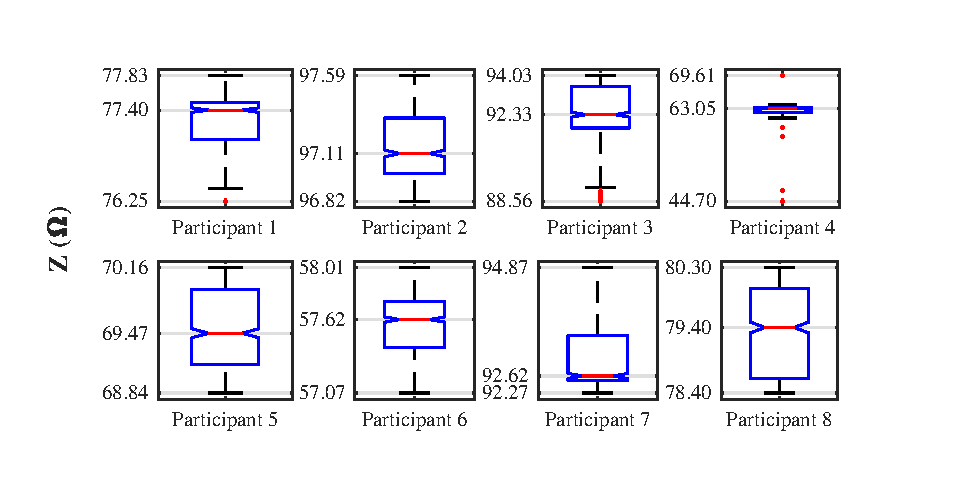
\includegraphics[width=0.85\textwidth,keepaspectratio]{figure_b_1}    
	\caption[Mean basal impedance box plot]{Mean basal impedance box plot of all the participants during the last \SI{3}{\minute} of the baseline regions 1, 3, 5 and 7.}
	\label{fig:Basal statistics} 
\end{figure}

Artefact motion triggered the outliers of the readings. As noticed from the plot, participants 1, 3 and particularly 4 presented the deviated points during the study. Additionally, participants 3, 4 and 8 exhibited the biggest distribution between interquartile values higher than \SI{1}{\ohm} (mean \SI{1.41(39)}{\ohm}). The remaining participants showed a distribution within first and third interquartile of about \SI{0.57(27)}{\ohm}. 

\subsection{Relation between geometry and mean basal impedance}
\label{section basal 2}
There are different aspects of the geometry which could impact the impedance reading. Several studies have demonstrated how the distance between electrodes affects readings on tissue \cite{yamamoto1992impedance, kun2000effects}. This study proves that the forearm's circumference and the distance between potential electrodes does influence the impedance measurement. Figure \ref{fig:C_vs_Z} shows an inverse relation between circumference and impedance (slope \SI{-0.072}{\centi\meter\per\ohm}). The smaller the  circumference of the forearm, the higher the resistivity. Meanwhile there is a direct relation between the distance between potential electrodes and the resistivity of the segment (slope \SI{0.055}{\centi\meter\per\ohm}) as depicted in \ref{fig:l_vs_Z}.

Moreover, when comparing total volume measured with the segment's mean resistivity (see figure \ref{fig:Ve_vs_Z}), the impedance tends to rise when there is a decline in the forearm's segment volume (slope \SI{-0.622}{\cubic\centi\metre\per\ohm}). This is congruent with the fact that when greater tissue is involved in the measurement, the path for current becomes more conductive, thus reducing the overall impedance. However, this cannot be seen as an entirely linear relationship since the impedance value can also be impacted by the amount of adipose tissue. When there are two different arms with same dimensions, the one with more fat content will produce a different basal impedance reading that its counterpart that has a higher muscular tone. 

\begin{figure*}[!b]
	\centering
	\begin{subfigure}[t]{0.48\textwidth}
		\centering
		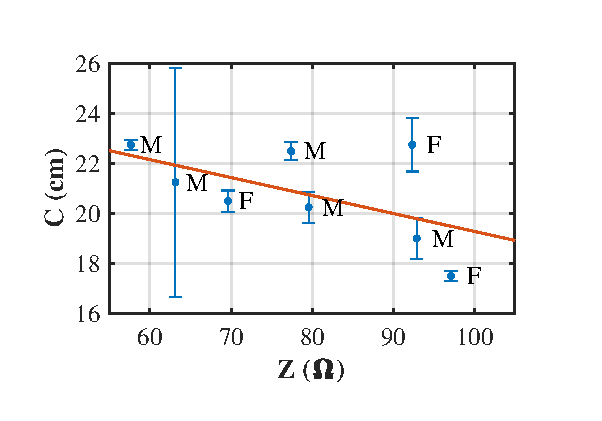
\includegraphics[width=7cm]{figure_b_2a}
		\caption{Relationship between forearm circumference and mean basal impedance}
		\label{fig:C_vs_Z}
	\end{subfigure}%
	~ 
	\begin{subfigure}[t]{0.48\textwidth}
		\centering
		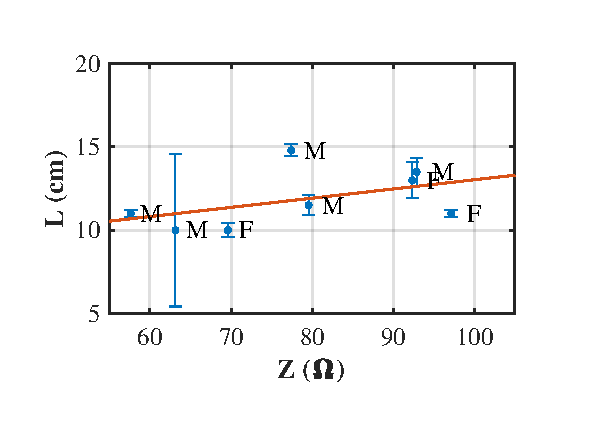
\includegraphics[width=7cm]{figure_b_2b}
		\caption{Relationship between distance sensing electrodes and mean basal impedance}
		\label{fig:l_vs_Z}
	\end{subfigure}
	~ 
	\begin{subfigure}[t]{0.48\textwidth}
		\centering
		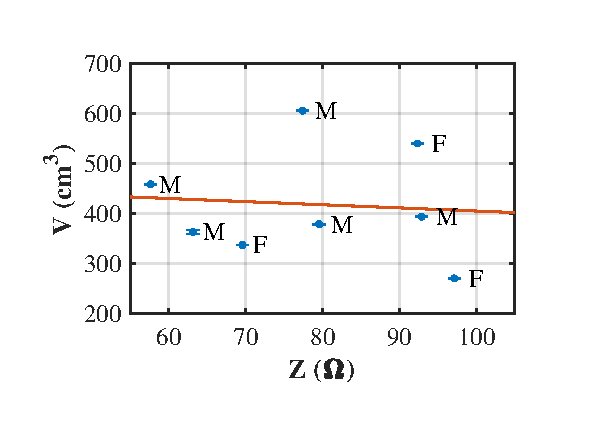
\includegraphics[width=7cm]{figure_b_2c}
		\caption{Relation between forearms segment volume and mean basal resistivity}
		\label{fig:Ve_vs_Z}
	\end{subfigure}
	\caption{Relation between circumference, length and total segment's volume and mean basal impedance}
	\label{fig:relation_geometry_vs_impedance}
\end{figure*}

\section{Basal impedance measurements}
\label{senction basal 3}
There are different artefacts that can alter the basal impedance during a measurement, such as motion or respiration movement \cite{pandey2006cancellation, swanson1983errors, ansari2010impedance, rosell1995reduction}. This section will analyse the extent of change in the basal impedance between the measurements. All participants were asked to stay still for the entire duration of the test. However, in practical terms, this is not entirely possible as staying still in the same position for a prolonged period of time can be quite tiresome. Inflating the cuff to a pressure above diastolic level may also cause discomfort to the participants, like tingling sensation or even pain. Thus, moving the limb to restore blood flow is a normal response of the body. The first \SI{2}{\minute} of the baseline impedance readings may be affected by the rearrangement of the participant's position, particularly after the upper arm's occlusion. Moreover, the restriction in blood flow also induced a physiological response which needed some time to revert to the baseline value. Hence, the baseline data after \SI{2}{\minute} is used for this analysis, thereby allowing some time for recovery. 

The data used for this analysis was compiled by extracting the lower envelope of the raw basal impedance. The command envelope in Matlab \cite{MATLAB:2016} allows the isolation of the desired signal. Figure \ref{fig:Basal Regions} displays the waveform extracted with the respective mean value for each region per participant. The region 1 is applicable to the time when the initial reference was recorded; in total, \SI{5}{\minute} were recorded but the last \SI{3}{\minute} of data was extracted right before the occlusion between \SIrange{120}{300}{\second}. This basal impedance is the reference to the other readings as it was unaffected by occlusion of any kind. The other sections of data correspond to region 3, which denotes the recovery after venous occlusion. The information extracted belongs to the time slot between \SIrange{ 600}{780}{\second}.  In a similar manner, the region 5 after partial arterial occlusion retrieves the last \SI{3}{\minute} of data between \SIrange{1080}{1260}{\second}. Finally, there is data after total occlusion in the region 7 between \SIrange{1560}{1740}{\second}.

Initially, the first thing that can be observed from this figure is the presence of oscillations in the baseline signal. This signal was present in all participants with subtle frequency variations between each region. The frequency was calculated by extracting the period of the signal as the difference between its peaks. On average, the frequency of the oscillation was \SI{0.0685(00027)}{\hertz}. At this point, it is not possible to establish whether this is a common noise from the instrument or a physiological response. In the literature, there is lack of sufficient information about impedance plethysmographic oscillations at this frequency band.  However, a study that used laser Doppler flowmetry found that the physiological measurements into this frequency spectrum may pertain to the sympathetic activity (\SIrange{0.02}{0.06}{\hertz}) \cite{kvandal2006low}. Further investigation needs to be undertaken in order to discover the roof of this signal. 

Secondly, it is evident that the motion artefact did make some alterations into the measurements. Participants 3 and 4 clearly displayed deviation from their mean values in region 2 and region 4, respectively. As a matter of fact, the figure had to be clipped off to adequately fit the waveform information. On the other hand, it becomes difficult to detect changes on partaker 1, but region 3 displayed significant variations when compared with other regions. Hence, this qualitative analysis confirms the quantitative results shown in figure \ref{fig:Basal statistics}.  

\begin{figure}[!htbp]  %fig:rb:all_participants
	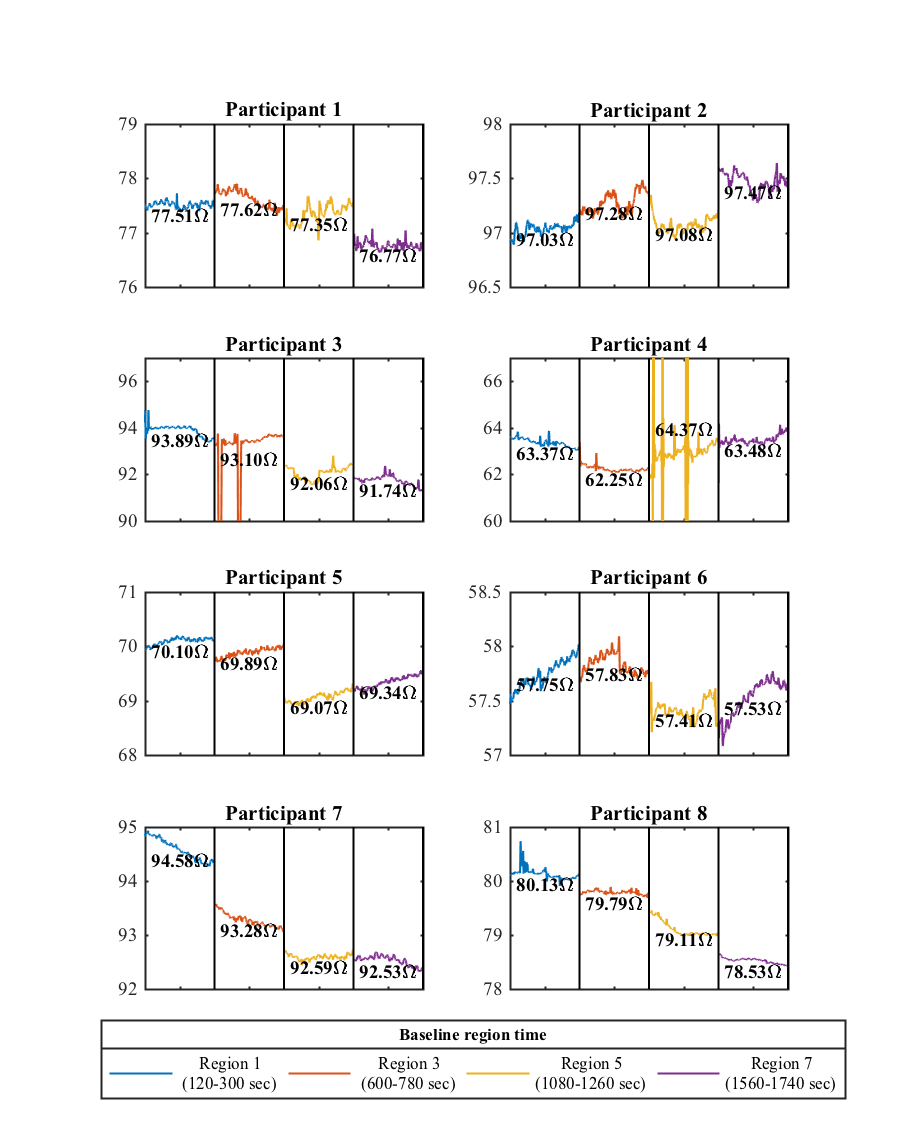
\includegraphics[width=\textwidth,keepaspectratio]{figure_b_3}    
	\caption[Measurements of the basal impedance during the whole study]{Basal impedance of all the participants during the entire study. The data has been divided into regions. The regions (1, 3, 5 and 7) in white colour represent baseline measurements. Similarly, the shaded areas (regions 2, 4 and 6) represent occlusive events.  }
	\label{fig:Basal Regions} 
\end{figure}

Lastly, it is also evident that there are variations on the baseline impedance between different regions. Furthermore, there is an absence of a clear trend on either the increase or decrease of basal impedance, with the exception of participants 7 and 8 where there a decrease on impedance is observed. Big gaps (< \SI{0.8}{\ohm}) between regions can be noticed on participant 5 and participant 7, respectively. It is important to determine whether the change of impedance is bigger than the time when VOP is performed. Therefore, the following section analyses the change of basal impedance whilst quantifying the changes. 


\section{Basal impedance change between regions}
\label{senction basal 3.1} 
The basal impedance signal contains noises that may deviate from the signal (from the baseline). As analysed in the previous section, the baseline changed between baseline regions. This section will quantify the error as compared to the basal impedance at the beginning of the experiment. 

Numerous factors could affect a bioimpedance reading. One of this is the change of impedance on the electrode-skin interface.  As described in section \ref{section impedance electrodes}, when there is a change in the geometry or the area of contact of the electrode, it gets converted into variations in the total impedance. Also, air pockets that could potentially form between the two elements could contribute to substantial changes in impedance.  Another contributing factor is the motion artefact. In this case, the movement of the skin and muscles creates different current paths. As a result, the basal impedance deviates from the baseline. 

In an in-vivo setting, it is difficult to keep a participant completely motionless for the entire duration of the experiment.  During each baseline, the upper arm's occlusion caused the participants to move and re-accommodate. Eventually, there was a change of impedance that will be analysed; it could be caused by that movement or perhaps a physiological response. 

The figure \ref{fig:delta percent} shows the deviation in percentage from the baseline in region 1.  Thus, the median impedance was the starting point in this region. The data was calculated by extracting the envelope of the impedance waveform. In the figure, each point denotes the median value of the resistance and the whiskers the range of data. It was the oscillatory component described in the previous section that triggered the major variations the resistance. The baseline impedance tended to decrease in majority of the participants, except number 2. 

The effect of the motion artefact can be observed on the large whiskers of some of the participants. For example, participants 3 and 4 demonstrated the bigger ones in region 3 and 5, respectively. Indeed, the data from participant 4 was clipped as the whiskers showed a huge variation of up to \SI{200}{\percent}. It is also important to note that only a few signals were able to return to baseline. For instance, the waveforms that experienced a variation below \SI{0.25}{\percent} included regions 3 and 4 of participant 1, participant 2 in region 5, participant 4 in region 7 and participant 6 in regions 3 and 7. The rest experienced changes of roughly \SIrange{-2.353}{0.441}{\percent} from the baseline region 1. 


\begin{figure}[!t]  %fig:rb:all_participants
	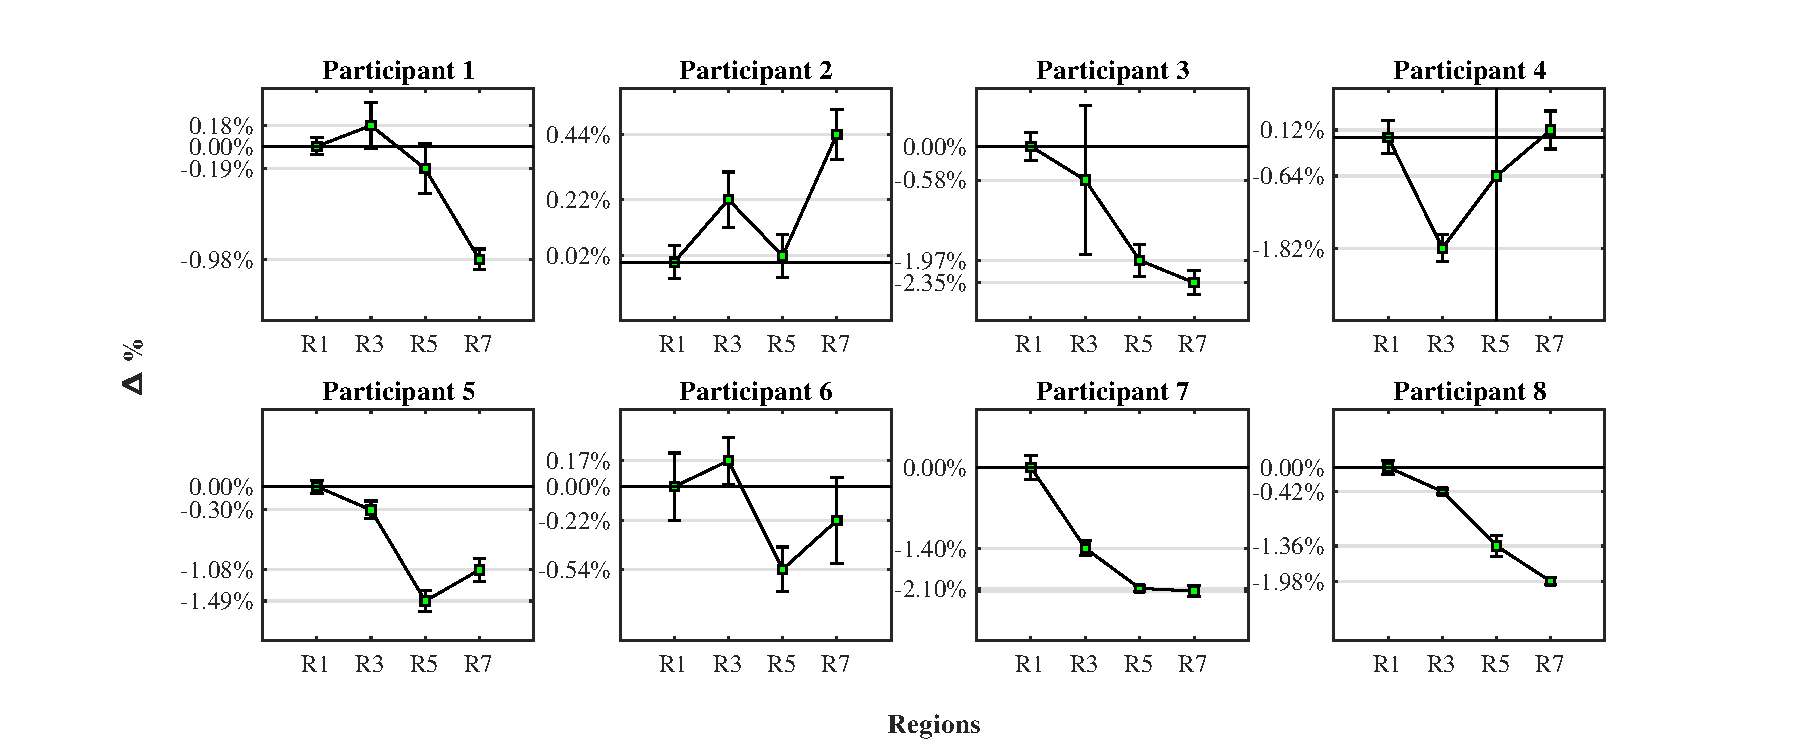
\includegraphics[width=\textwidth,keepaspectratio, trim={2cm 0cm 3cm 0cm},clip]{figure_b_4}    
	\caption[Percentile change of baseline impedance]{Deviation of the basal impedance for all the participants compared to region 1. Each plot shows how much the impedance increase or decrease against the reference value for regions 3, 5 and 7. }
	\label{fig:delta percent} 
\end{figure}

The table \ref{tbl:change imepdance} illustrates the range and mean of changes of impedance for all the participants. The average impedance of the entire study was \SI{-0.6384}{\percent} with a range of about \SI{1.5264}{\percent}. Certainly, participants 1, 2 and 7 illustrated the least impedance change with less than \SI{0.25}{\percent}, whereas the second one increased and others decreased.  A change occurring between \SIrange{0.25}{1}{\percent} was experienced by participants 4, 5 and 8. Finally, participants 3 and 7 recorded the biggest change of impedance of over \SI{1}{\percent}. 

\begin{table}[!htbp]
	\caption[Range and mean change of impedance of each participant]{Mean and range of the impedance change for each participant.}
	\label{tbl:change imepdance}
	\centering \small
	\begin{tabular}{lcc}
		\toprule
		&\textbf{range ($\Delta \%$)}
		&\textbf{mean ($\Delta \%$)} \\ \midrule
		Participant 1    &     \SI{1.157}{\percent}    &     \SI{-0.247}{\percent}    \\  
		Participant 2    &     \SI{0.441}{\percent}    &     \SI{0.170}{\percent}    \\  
		Participant 3    &     \SI{2.353}{\percent}    &     \SI{-1.226}{\percent}    \\  
		Participant 4    &     \SI{1.939}{\percent}    &     \SI{-0.584}{\percent}    \\  
		Participant 5    &     \SI{1.489}{\percent}    &     \SI{-0.719}{\percent}    \\  
		Participant 6    &     \SI{0.707}{\percent}    &     \SI{-0.148}{\percent}    \\  
		Participant 7    &     \SI{2.147}{\percent}    &     \SI{-1.412}{\percent}    \\  
		Participant 8    &     \SI{1.979}{\percent}    &     \SI{-0.940}{\percent}    \\ 
		\bottomrule 
	\end{tabular}
\end{table}

\section{Statistical analysis of basal impedance}
\label{section basal 4} 
Identifying when the basal impedance is outside normal levels requires a statistical analysis. By using the entire percentage deviation ($\Delta \%$) from the initial baselines as the data range, it was calculated as the normal probability density function (PDF). Using the Matlab command \textit{normfit} the normal distribution was computed from the $\Delta \%$. The calculation returned a $\mu = -0.6384$ and a $\sigma = 0.8518$. By plotting the probability distribution function, it can be seen how the probability was distributed. Then by using the $\sigma$ that was obtained from the data, a new PDF was calculated which centred at $\mu = 0$. Therefore, the PDF produces a similar data distribution where the confidence band (\SI{95}{\percent}) was calculated at $\pm 1.96 \times\sigma$.

Figure \ref{fig:basal pdf} shows the PDF obtained from the data and the new one calculated. The yellow plot shows the confidence area from the baseline. Therefore, the confidence band is located between $\Delta \% = \pm 1.66 \%$. In other words, all changes of impedance within this confidence band can be considered to be statistically important and is located within normal limits. 

By comparing the results shown from the PDF, most participants were found to be within that range. Nevertheless, some partaker's regions do not lie within this confidence band. These include regions 5 and 7 in participants 3 and 7, region 3 of participant 4 and region 7 of participant 8.

\begin{figure}[!htbp]  %fig:rb:all_participants
	\centering
	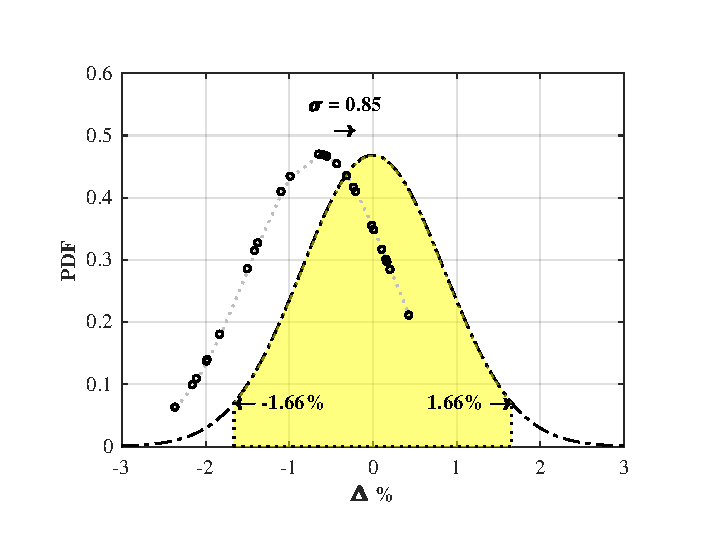
\includegraphics[width=12cm,keepaspectratio, trim={0cm 0cm 0cm 0cm},clip]{figure_b_5}    
	\caption[Percentil change of baseline imepdance]{Deviation of the basal impedance for all the participants compared to region 1. Each plot shows the extent of increase or decrease in the impedance against the reference value for regions 3, 5 and 7. }
	\label{fig:basal pdf} 
\end{figure}


\section{Change of basal impedance during occlusions}
\label{section occlusion 1}
From the data obtained in the experimental procedure, different data regions were extracted in accordance to the kind of occlusion applied as depicted in \ref{fig:pressure applied}. The data were separated in this section into the readings from venous occlusion, partial arterial occlusion (PAO) and total blockage. 

Data analysis needs to be performed on the basis of basal impedance. Similarly, as mentioned in the previous chapter, the arterial pulses were eliminated from the signal. Only, the lower envelope of this impedance signal was used to perform this investigation. 

The data set for this study was subdivided in the following manner: two minutes of data before the occlusion as the baseline reference and three minutes of occlusion followed by two minutes of data after releasing the cuff's pressure. 

\subsection{Basal impedance shift during venous occlusion}
\label{section occlusion 1.1}
As expected, the basal impedance declined while performing venous occlusion in each participant. As confirmed by figure \ref{fig:venous statistics impedance}, all the partakers witnessed a decline in their basal impedance in region 2 of the experiment. The boxplot illustrates that three regions that were part of this study. The data of the region 1 (\textit{R1}) were the last \SI{2}{\minute} of the initial baseline (\SIrange{180}{300}{\second}). Thereafter, it is the venous occlusion in region 2 (\textit{R2}) during \SI{3}{\minute} at the pressure levels described by the column \textit{occlusion 1} in \ref{tbl: venous occlusions}. This makes it clear that the median resistance value decreased. While analysing this candle-stick, it can be surmised that bigger the distribution of the upper and lower quartile, the greater the resistance decline as registered by most other participants, with the exception of participant 6 whose impedance measurement settled quickly. After releasing the cuff's air, the median impedance in region 3 was expected to return to a value close to the initial baseline. However, partakers 3 and 4 were unable to recover completely. While their resistance values improved for a few seconds, they continued to reduce below the lower whisker of region 2. Meanwhile participants 1 rose over the initial baseline median. Participant 3 was the only one who showed a return to baseline. 

\begin{figure}[htbp]
	\centering
	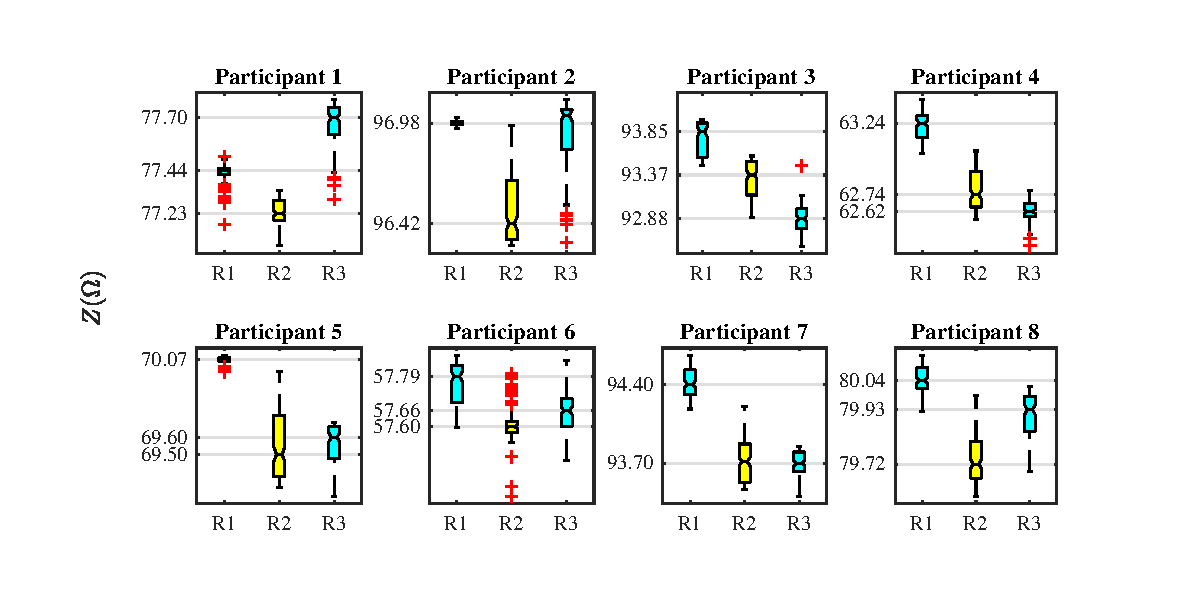
\includegraphics[width=15cm,keepaspectratio]{figure_vop_1}    
	\caption[Change of impedance during venous occlusion]{Box plot showing the statistical change of impedance in $\Omega$ during venous occlusion. The cyan boxplot represents the baseline before (Region 1) and after (Region 3) the occlusion. The yellow marker is the impedance during venous occlusion (Region 2).}
	\label{fig:venous statistics impedance}
\end{figure}  

Figure \ref{fig:venous occlusion impedance} illustrates that the deviation of impedance in terms of the changes in percentage of impedance ($\Delta Z\%$) from the median baseline in region 1. The shaded area represents the venous occlusion between \SIrange{300}{400}{\second}. These dots are the points of foot of the signal equivalent to ($R_B$). This signal was smoothed using the command \textit{smooth} in Matlab which assigns a lower weight to outliers within the regression \cite{MATLAB:2016}. This method assigns zero weight to data outside of the six mean absolute deviations. By doing so, it eliminates most of the rapid variations of impedance triggered by motion artefact. 

\begin{figure}[htbp]
	\centering
	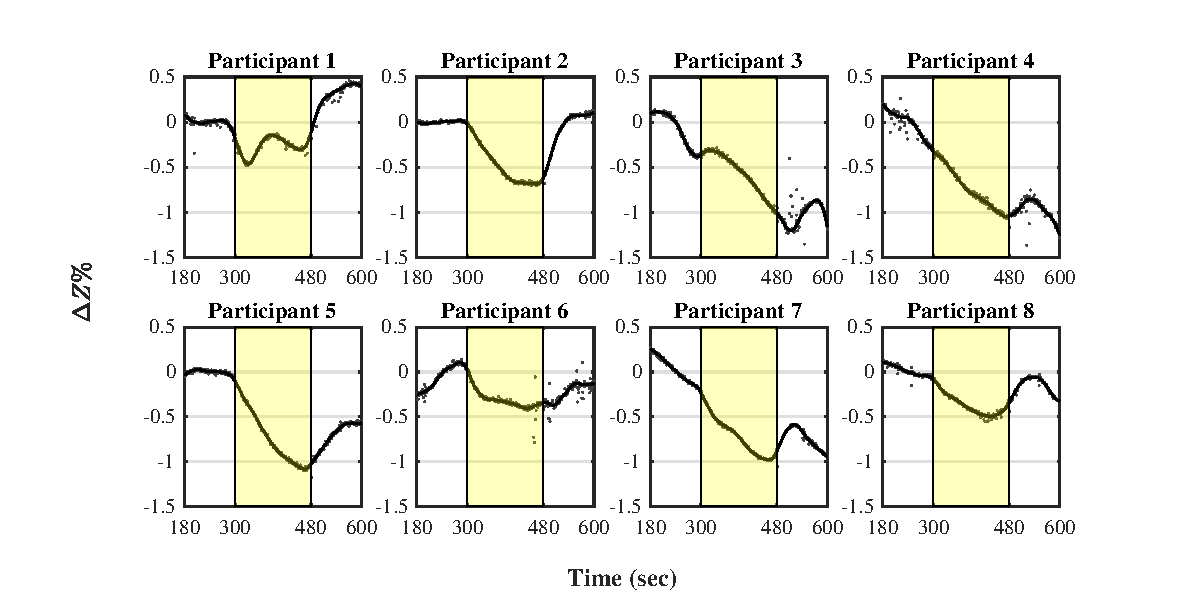
\includegraphics[width=15cm,keepaspectratio]{figure_vop_2}    
	\caption[Percentile variation of impedance during venous occlusion]{Percentile change of impedance during venous occlusion. The reference baseline is the average baseline impedance during the last \SI{2}{\minute} before the venous occlusion.}
	\label{fig:venous occlusion impedance}
\end{figure} 

The figure clearly reveals a linear trend during venous occlusion for majority of the subjects. Nonetheless, the resistance of participant reduced immediately upon occlusion, but the participant moved his arm a minute later to reverse the trend. Subsequently, the impedance continued to decline again. Furthermore, participant 6 also showed a similar response when the individual moved his arm, but the resistance settled instead of reversing the trend in this case. Interestingly, participant 2 showed a saturation point after a few seconds, which was specific for this subject. 

The table \ref{tbl:vop delta impedance} summarises the changes of impedance caused during the venous occlusion. The average median of the resistance decline from the baseline value stood at roughly \SI{-0.546(0076)}{\%}, where participants 4, 5 and 7 recorded the biggest losses of impedance (>\SI{0.5}{\%}). The column \textit{Change} on the same table shows the impedance difference from the point of initial occlusion to the minimum point of the smooth curve, which was calculated using equation \ref{eq:DeltaZ}. During the venous occlusion the whole slope was seen to record a variation of \SI{0.658(0230)}{\percent}.

\begin{align}
	\label{eq:DeltaZ}
	\Delta Z\%_T = \Delta Z\%_{300 sec} - \Delta Z\%_{min}
\end{align}


\begin{table}[htbp]
	\caption[Statistical analysis of the percentile change of impedance during venous occlusion]{Statistical analysis of the percentile change of impedance during venous occlusion. The data denotes the median percentile change of impedance per participant, the maximum and minimum value of the occlusion, and the difference between these two peak values.}
	\label{tbl:vop delta impedance}
	\centering
	\begin{tabular}{l@{\hspace{1cm}}
			S[table-format=-1.2]@{\,\( \pm \)\,}
			S[table-format=1.2]
			c
			c
			c}
		\toprule
		&\multicolumn{2}{c}{\textbf{Median}}  
		&\textbf{Max} 
		&\textbf{Min}
		&\textbf{Change} \\ 
		&\multicolumn{2}{c}{\textbf{[$\Delta Z \%$]}}
		&\textbf{[$\Delta Z \%$]}
		&\textbf{[$\Delta Z \%$]}
		&\textbf{[$\Delta Z \%$]}\\\midrule
		Participant 1 & -0.26 & 0.09 & -0.20 & -0.47 & 0.26 \\ 
		Participant 2 & -0.58 & 0.21 & -0.03 & -0.69 & 0.66 \\  
		Participant 3 & -0.51 & 0.22 & -0.35 & -1.00 & 0.66 \\  
		Participant 4 & -0.79 & 0.22 & -0.32 & -1.06 & 0.74 \\ 
		Participant 5 & -0.82 & 0.30 & -0.11 & -1.09 & 0.98 \\  
		Participant 6 & -0.33 & 0.09 &  0.03 & -0.41 & 0.43 \\  
		Participant 7 & -0.72 & 0.22 & -0.22 & -0.98 & 0.77 \\  
		Participant 8 & -0.40 & 0.11 & -0.09 & -0.50 & 0.41 \\  
		\bottomrule
	\end{tabular} 
\end{table}		

It is tempting to observe the immediate change of impedance as soon as the venous occlusion occurs. The capability of impedance plethysmography device of detecting venous occlusion in all participants is remarkable and almost instantaneous. As soon as the blockage occurs, the impedance reduces for some time. If motion does not bring about changes in the trend, some of them could reach the saturation point, as seen in the case of participant 2. However, it is also apparent that other signals reached a point of saturation, signalling a decline of impedance in an exponential trend than linear. 

This effect can be summarised in figure \ref{fig:venous occlusion change}. The plot describes the change of impedance in time ($dZ/dt$) against some data points (beats) during the venous occlusion. Accordingly, 10 data points of $R_B$ synchronised with the heart cycle were clustered computing $dZ/dt$. This differential value is equivalent to the velocity of the change in basal impedance per second (\si{\ohm\per\second}). In general, the average impedance all along the occlusion was observed at \SI{-0.0026(00018)}{\beats}.

\begin{figure}[htbp]
	\centering
	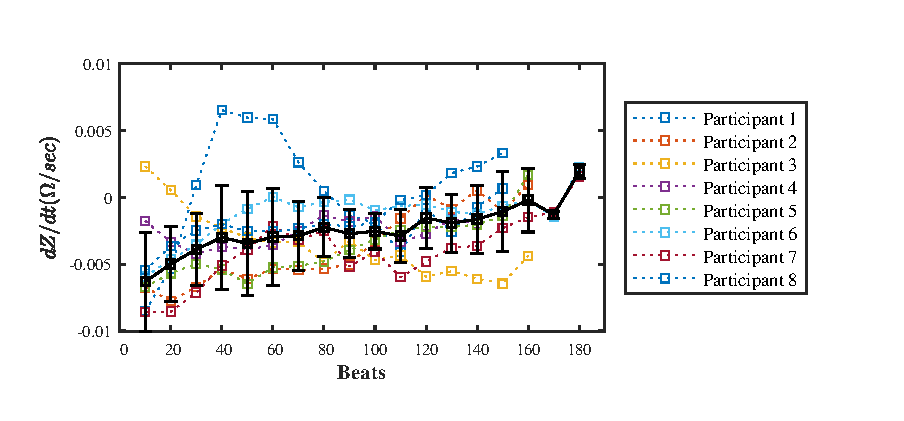
\includegraphics[width=15cm,keepaspectratio]{figure_vop_3}    
	\caption[Rate of change of impedance per 10 heartbeats during venous occlusion]{Speed of change of impedance in time ($dZ/dt$) per every 10 heartbeats during venous occlusion. The colour lines represent the data per each participant. The dark bold line is the mean of all the measurements.}
	\label{fig:venous occlusion change}
\end{figure}

Based on the figure, it can be surmised that during the first 10 beats, there is a higher drop of impedance as compared to the last data points. Indeed, the rate of change of resistance during the first 10 beats was on average \SI{-0.0063(00037)}{\Omega\per\second}. After 90 beats, the result of this derivation was more than halved to an average of \SI{-0.0027(00018)}{\Omega\per\second}. At 160 beats, the ratio was reduced to merely \SI{-0.0002(00024)}{\Omega\per\second}. The final data points (180 beats) exhibited a reversion of the trend (\SI{0.0019(0005)}{\Omega\per\second}). However, this is because only a few participants were able to achieve that amount of heart beats.  Moreover, at this point, some data were already returning to the baseline because the cuff could have been released a few seconds earlier.  

\subsection{Basal impedance change during partial arterial occlusion}
\label{section occlusion 1.2}
The same analysis performed on the VOP was applied to the partial arterial occlusion. A partial restriction of arterial blood flow is achieved by mechanically occluding the upper arm between diastolic and systolic pressures. The load levels used to create these occlusions are detailed on the column \textit{occlusion 2} in the table \ref{tbl: venous occlusions}. Similar time lapses were incorporated to analyse the data, the last \SI{2}{\minute} of the region 3 (\SIrange{660}{780}{\second}), the entire partial arterial blockage in region 4, \SI{3}{\minute} between \SIrange{780}{960}{\second}, followed by \SI{2}{\minute} of return to the baseline after releasing the pressure of the cuff in region 5 (\SIrange{960}{1080}{\second}).

Occluding the blood flow at this pressure level induced a sense of discomfort among participants; some of them felt numbness in their arms during the experiment. Therefore, some partakers moved their arms like participant 1. In the case of others, the duration of occlusion had to be shortened as was done in the case of participant 4 where the occlusion occurred subsequently (\SIrange{840}{960}{\second}) because ECG sensors had to be relocated and participant 8 who asked to terminate the blockage a minute earlier (\SIrange{780}{900}{\second}). 

During this kind of occlusion, there is no venous return. In addition, the inflow is slightly restricted as well. Indeed, the occlusion constricts the brachial artery where only a small amount of blood passes through the obstruction. Moreover, the blood flow becomes turbulent after the cuff's constriction.  Due to the venous occlusion, the arm is expected to increase its volume as blood pools within the forearm to reduce the basal impedance. 

Figure \ref{fig:partial arterial statistics impedance} confirms the reduction of the basal impedance all along the partial arterial occlusion. When compared to VOP, the box-plot shows a higher upper and lower quartile distribution for majority of the participants in region 4, owing to a continued decline in basal impedance during that occlusive action. However, partaker 4 depicted a significant number of outliers primarily caused by motion artefact. Only a few participants were able to get back close to baseline resistance, such as participants 2 and 7. Interestingly, some members showed a swift recovery in region 5. For instance, the large data distribution across participants 1, 2, 4, 6, 7 and 8 suggests a quick trend to return to the baseline. However, it generally seems that a longer recovery time is required in order to return to an impedance value close to the baseline after partial arterial occlusion. 

\begin{figure}[htbp]
	\centering
	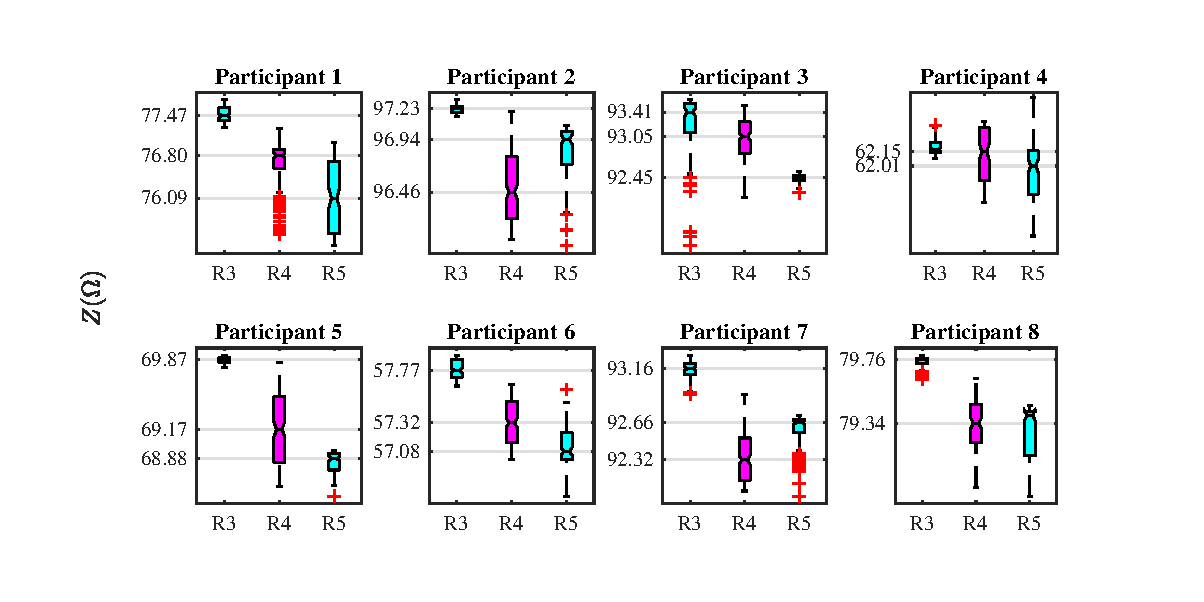
\includegraphics[width=15cm,keepaspectratio]{figure_vop_4}    
	\caption[Change of impedance during partial arterial occlusion]{Box plot of the statistical change of impedance in $\Omega$ during partial arterial occlusion. The cyan marker represents the baseline before (Region 3) and after (Region 5) the occlusion. The magenta marker is the impedance during partial arterial occlusion (Region 4).}
	\label{fig:partial arterial statistics impedance}
\end{figure}  

Through a qualitative analysis of the change of impedance by percentage from baseline region 3, figure \ref{fig:arterial occlusion impedance} shows a linear trend during the cuff's pressure exerted in region 4. It can be seen that the impedance decline is more pronounced than the one recorded from venous occlusion (see figure \ref{fig:venous occlusion impedance}). In participant 1, the motion artefact becomes more evident, the step drop of basal impedance immediately before releasing the cuff's pressure is a reflection of his forearm's muscular movement. In this case, it is evident that the arm movement augmented the change of impedance throughout the occlusion. While other participants also experienced motion artefact, the change of impedance was within a few heart beats. For example, participant 2 only showed a data point off the smooth line. However, in participants 3 and 4, the amount of data points off the soft signal was significantly higher. In summation, majority of the participants described a straight drop of impedance, particularly linear in participants 2 and 5. 

After releasing the cuff's pressure, it is evident that most of the signals change their slope. The only member that did not reflect this change was participant 3. This impedance correction is indicative of a restoration of blood circulation and a decline in the forearm's volume. Moreover, a lack of apparent settling impedance value can be observed, barring participants 7 and 8. In general, this change in trend also confirms that the body might require a longer time to recover after the partial arterial occlusion.

\begin{figure}[htbp]
	\centering
	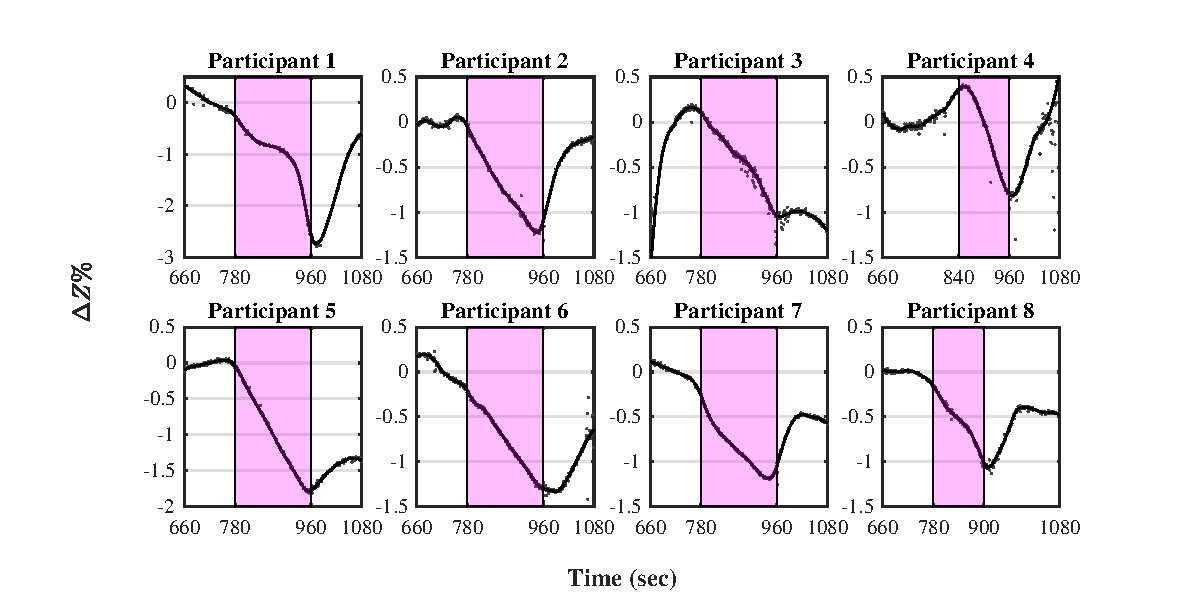
\includegraphics[width=15cm,keepaspectratio]{figure_vop_5}    
	\caption[Percentile variation of impedance during partial arterial occlusion]{Percentile change of impedance during partial arterial occlusion using as reference average baseline impedance during the last \SI{2}{\minute} before the occlusion.}
	\label{fig:arterial occlusion impedance}
\end{figure}  

Table \ref{tbl:AO delta impedance} reports the variations in percentage from the baseline impedance in region 3 in greater depth. The median impedance decline from the baseline was approximately \SI{-0.783(0324)}{\percent}. However, participant 4 exhibited a lower median value since the initial impedance value stood above the baseline average at \SI{0.34}{\percent}. Evidently, there is a greater reduction of impedance or an increase in the forearm's volume as opposed to VOP. The median change of impedance from the maximum to the minimum value was nearly \SI{1.133(0482)}{\percent} which is about double when compared with venous occlusion. A physiological response might have caused this increase in volume. The blood pooling could not have caused this volume increase given that the arterial blood flow was restricted, which lowered the amount of blood to enter the forearm segment. 

\begin{table}[htbp]
	\caption[Statistical analysis of the percentile change of impedance during partial arterial occlusion]{Statistical analysis of the percentile change of impedance during partial arterial occlusion. The data represents the median percentile change of impedance per participant, the maximum and minimum value during the occlusion and the difference between these two peak values.}
	\label{tbl:AO delta impedance}
	\centering
	\begin{tabu}{l@{\hspace{1cm}}
			S[table-format=-1.2]@{\,\( \pm \)\,}
			S[table-format=1.2]
			c
			c
			c}
		\toprule
		&\multicolumn{2}{c}{\textbf{Median}}  
		&\textbf{Max} 
		&\textbf{Min}
		&\textbf{Change} \\ 
		&\multicolumn{2}{c}{\textbf{[$\Delta Z \%$]}}
		&\textbf{[$\Delta Z \%$]}
		&\textbf{[$\Delta Z \%$]}
		&\textbf{[$\Delta Z \%$]}\\\midrule
		Participant 1 & -0.85 & 0.50 & -0.28 & -2.56 & 2.29 \\  
		Participant 2 & -0.80 & 0.35 & -0.05 & -1.23 & 1.18 \\  
		Participant 3 & -0.38 & 0.32 &  0.10 & -1.04 & 1.14 \\  
		Participant 4 & -0.03 & 0.41 &  0.34 & -0.78 & 1.13 \\  
		Participant 5 & -1.01 & 0.54 & -0.04 & -1.80 & 1.76 \\  
		Participant 6 & -0.77 & 0.33 & -0.21 & -1.30 & 1.09 \\  
		Participant 7 & -0.90 & 0.26 & -0.25 & -1.19 & 0.93 \\  
		Participant 8 & -0.53 & 0.22 & -0.15 & -1.01 & 0.85 \\  
		\bottomrule
	\end{tabu} 
\end{table}	

\begin{figure}[!t]
	\centering
	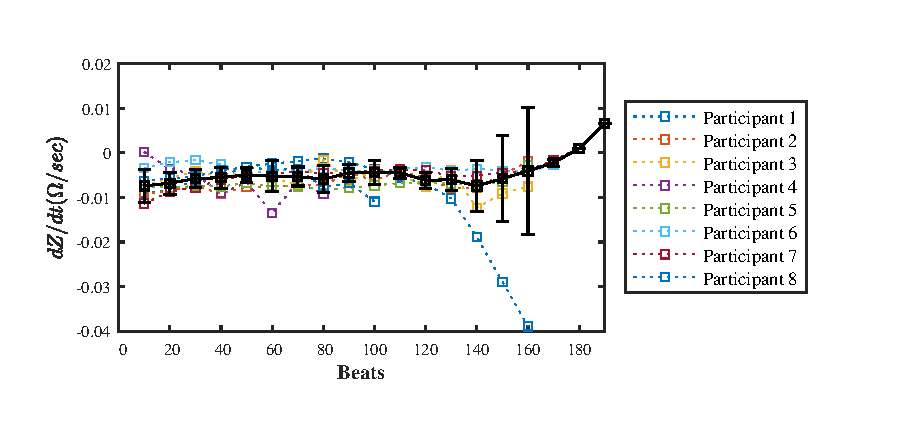
\includegraphics[width=15cm,keepaspectratio]{figure_vop_6}    
	\caption[Rate of change of impedance per 10 heartbeats during partial arterial occlusion]{Speed of change of impedance in time per every 10 heartbeats during partial arterial occlusion. The colour lines represent the data per each participant. The dark bold line is the mean of all the measurements.}
	\label{fig:arterial occlusion change}
\end{figure}  

The calculation of the velocity of the change of impedance ($dZ/dt$) displayed a similar exponential response as was seen in VOP. Figure \ref{fig:arterial occlusion change} shows the calculation of these points across all participants. The plot indicates that the first 10 beats of changes on a ratio average of \SI{-0.0074(00037)}{\Omega\per\second} was the largest acceleration. Subsequently, between 20 and 110 beats, the velocity stabilised to \SI{-0.0053(00007)}{\Omega\per\second}. After this apparent settling, a new increase was witnessed in the differentiation. However, it seems to have been aided by the motion artefact seen on participant 1 for a few beats.

\subsection{Basal impedance variation during total occlusion}
\label{section occlusion 1.3}
The blood supply towards the forearm was completely blocked by inflating the cuff above systolic pressure in this study \SI{20}{\mmHg} above this point. The column \textit{occlusion 3} in the table \ref{tbl: venous occlusions} illustrates the pressure level applied for the research. The data regions involved in this part of the investigation were regions 5, 6 and 7. As was the case with previous occlusions analysis, the last 2 minutes of the data sourced from region 5 were used as impedance baseline (between \SIrange{1140}{1260}{\second}). The cuff was then inflated to accomplish complete blood flow obstruction; the occlusion was maintained for \SI{3}{\minute} between \SIrange{1260}{1440}{\second}. Finally, the cuff's air was released immediately, and the readings were taken for further \SI{2}{\minute}.

This test caused plenty of discomfort to most participants. Numbness and an unwillingness to move their limb was commonly seen in all the participants. Hence, they ended up moving their arms on a voluntary basis. Due to the absence of blood flow or pooling during this aspect of the experiment, small impedance variations were expected. Additionally, the mean restive value would be equivalent to the impedance of the tissue's components within the segment in addition to the impedance of the residual blood within the forearm. However, when a change of resistivity takes place, this is mostly caused by the participant's re-accommodation as opposed to a physiological variable. 

Figure \ref{fig:total arterial statistics impedance} shows how the impedance changes during the total occlusion. Initially, it can be seen that there was an absence of consensus on the signal trend all along the occlusion, as seen in the previous tests.  Some of the participants reflected a small reduction in their median impedance, such as study members 1, 4, 5, 6 and 8. Meanwhile the rest experienced a slight increase. In addition, the trend of signal during the occlusion is ambiguous; different signals have different data distribution points. For instance, participants 1 and 7 displayed a large data distribution, indicating a constant change of their median impedance. In contrast, the rest exhibited a data distribution centred in the median, illustrating a little impedance variation during the occlusion. Only participant 5 exhibited a significant number of outliers, denoting swift changes at one point of the measurement. In general, there is no linear trend, as reported by the other kinds of occlusions. 

\begin{figure}[!hpb]
	\centering
	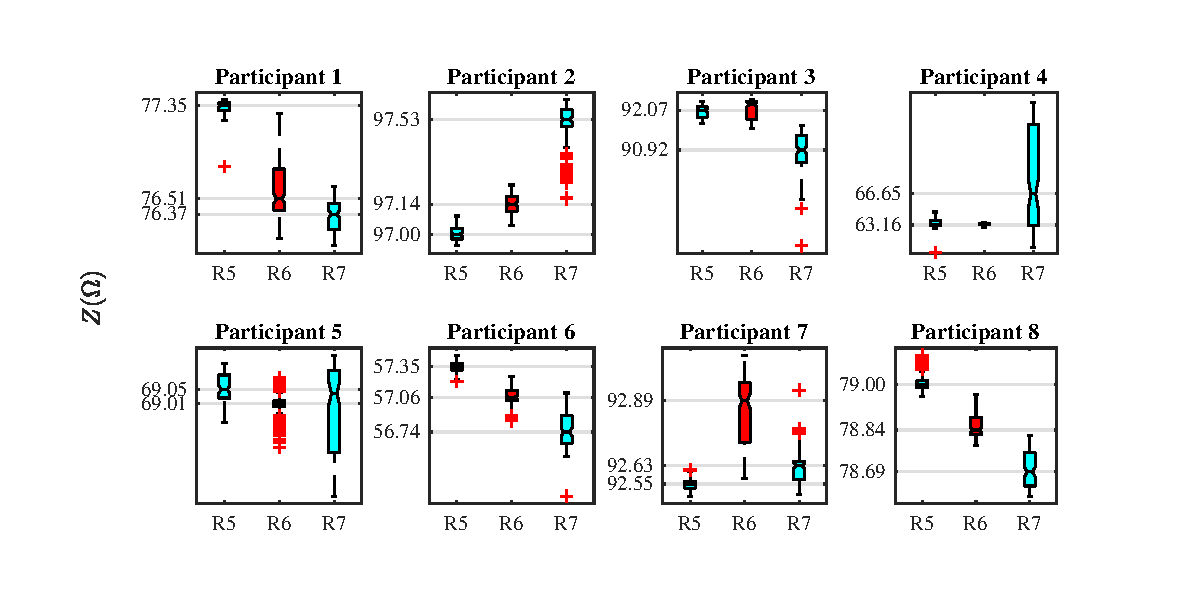
\includegraphics[width=15cm,keepaspectratio]{figure_vop_7}    
	\caption[Change of impedance during total occlusion]{Box plot of statistical change of impedance in $\Omega$ during total occlusion. The cyan marker represents the baseline before (Region 5) and after (Region 7) the occlusion. The red marker denotes the impedance during total occlusion (Region 6).}
	\label{fig:total arterial statistics impedance}
\end{figure} 

After releasing the cuff's pressure, no definite trend was observed in the direction of the impedance. Some participants displayed an increase of resistivity. However, participants 4 and 5 exhibited exaggerated changes in impedance. While the nature of this rare variation remains unclear, it could be attributed to the limb movement after the occlusion. Moreover, there was no swift change of impedance as was experienced in other types of occlusions. This is congruent with the fact that no blood rushed in or out of the forearm.

By analysing the variation of impedance during the occlusion as compared to the baseline (region 5), the magnitude and direction of the resistivity change can be seen. Evidently, participant 1 displayed the biggest and continuous impedance decrease, which is unusual for this type of occlusion. Another unexpected resistivity response was shown by participant 7 where his impedance increased, albeit slightly.  

The table \ref{tbl:TO delta impedance} illustrates the impedance changes during the occlusion in detail. The median impedance during total occlusion was \SI{-0.135(0441)}{\percent} which is fairly close to zero. However, the sign of column \textit{median} indicates that five out of eight exhibited a negative trend in the impedance direction to indicate resistivity loss. In fact, most of the measurements were below \SI{0.5}{\percent}; only participants 1 and 5 exhibited higher changes of impedance. By calculating the $\Delta \%$ from the maximum and minimum changes (column \textit{Change}), it can be surmised that only participant 1 showed a change greater than \SI{1}{\percent}, between \SIrange{0.5}{1}{\percent}, participants 3 and 6 displayed this data range, whereas the rest were below \SI{0.5}{\percent}. In general, the changes described by total occlusion were found to be significantly lower than the other occlusions, indicating a minimum increase of volume. For instance, partakers 2 and 5 median impedance signified a clear illustration of this. Some impedance changes were presented in some measurements which can be associated with a muscular activity. 

\begin{figure}[htbp]
	\centering
	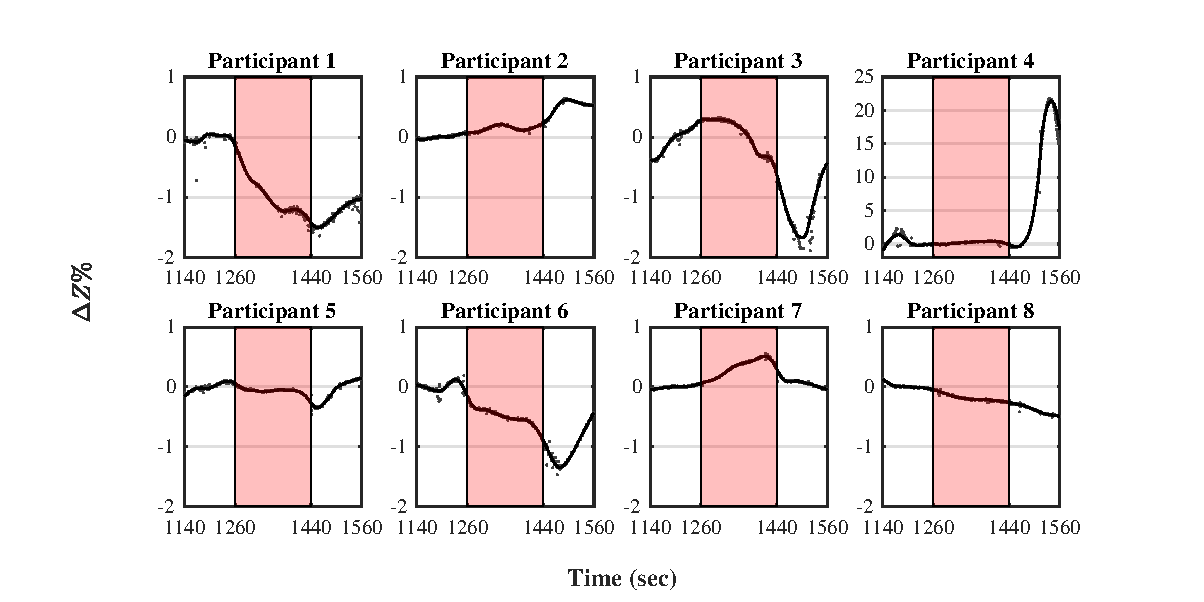
\includegraphics[width=15cm,keepaspectratio]{figure_vop_8}    
	\caption [Percentile variation of impedance during total occlusion]{Percentile change of impedance, using as reference average baseline impedance all along the last \SI{2}{\minute} before the total occlusion.}
	\label{fig:total occlusion imepdance}
\end{figure} 

\begin{table}[htbp]
	\caption[Statistical analysis of the percentile change of impedance during total occlusion]{Statistical analysis of the percentile change of impedance during total occlusion. The data signifies the median percentile change of impedance per participant, the maximum and minimum value during the occlusion, and the difference between these two peak values.}
	\label{tbl:TO delta impedance}
	\centering
	\begin{tabu}{l@{\hspace{1cm}}
			S[table-format=-1.2]@{\,\( \pm \)\,}
			S[table-format=1.2]
			c
			c
			c}
		\toprule
		&\multicolumn{2}{c}{\textbf{Median}}  
		&\textbf{Max} 
		&\textbf{Min}
		&\textbf{Change} \\ 
		&\multicolumn{2}{c}{\textbf{[$\Delta Z \%$]}}
		&\textbf{[$\Delta Z \%$]}
		&\textbf{[$\Delta Z \%$]}
		&\textbf{[$\Delta Z \%$]}\\\midrule
		Participant 1 & -1.09 & 0.33 & -0.14 & -1.38 & 1.24 \\  
		Participant 2 &  0.14 & 0.04 &  0.07 &  0.07 & 0.00 \\  
		Participant 3 &  0.18 & 0.28 &  0.30 & -0.50 & 0.81 \\  
		Participant 4 &  0.21 & 0.16 &  0.05 & -0.14 & 0.19 \\  
		Participant 5 & -0.06 & 0.05 &  0.05 & -0.23 & 0.28 \\  
		Participant 6 & -0.51 & 0.14 & -0.15 & -0.89 & 0.75 \\  
		Participant 7 & -0.36 & 0.15 &  0.05 &  0.05 & 0.00 \\  
		Participant 8 & -0.21 & 0.06 & -0.05 & -0.27 & 0.22 \\  
		\bottomrule
	\end{tabu} 
\end{table}	

Figure \ref{fig:total occlusion change} illustrates the analysis of velocity rate ($dZ/dt$) which is altered by the basal impedance. Evidently, the basal impedance of participant 1 decreased swiftly when compared to the rest. Moreover, participant 3 witnessed a rapid impedance drop between \SIrange{80}{140}{\beats}. In general, the average velocity for the total occlusion procedure stood at around \SI{-0.00061(000170)}{\Omega\per\second} which is considerably small when compared with occlusions. However, at the beginning of this occlusion, a modest increase was seen in the velocity; the average for the first \SI{10}{\beats} stood at around \SI{-0.0027(00052)}{\Omega\per\second}. Subsequently, it stabilised close to the median value of the entire measurements until \SI{140}{\beats}. Nonetheless, between \SIrange{140}{180}{\beats}, an increase was seen in the velocity due to the contribution of negative trends before releasing the occlusion. 

\begin{figure}[htbp]
	\centering
	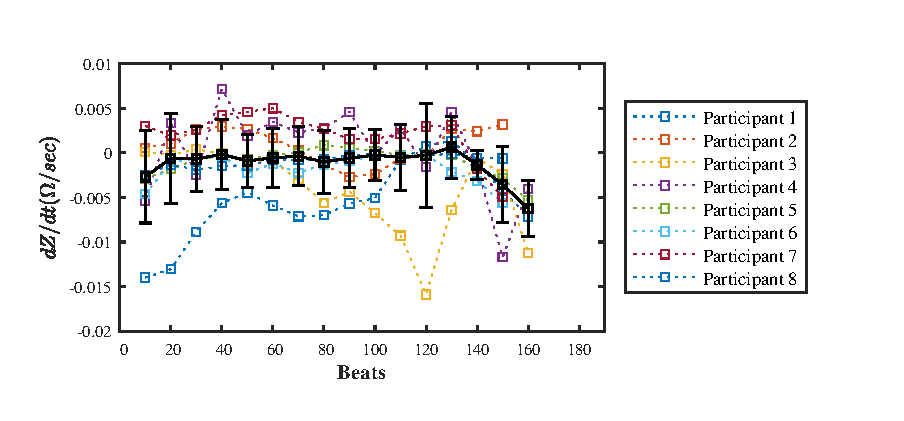
\includegraphics[width=15cm,keepaspectratio]{figure_vop_9}    
	\caption[Rate of change of impedance per 10 heartbeats during total occlusion]{Speed of change of impedance over time per every 10 heartbeats during the total occlusion. The colour lines denote the data per each participant. The dark bold line represents the mean of all the measurements.}
	\label{fig:total occlusion change}
\end{figure} 

\section{Conclusion}
\label{section basal conclusion} 

There are different bodily tissues that contribute to the impedimetric signal, such as fat, muscle, blood and bone. Most of these organs or tissues entail intrinsic impedances. The sum of all these resistive values is referred to as basal impedance. The collected data showed that the geometry of the forearm segment changed the impedance reading, exhibiting an inverse relation between the volume of segment and the average impedance. The device took measurements within the expected ranges of a human forearm. However, motion artefact or the interface electrode-skin, may have contributed to the change in resistance value of the measurement. The basal impedance varied from the median measurement in average \SI{-0.6384}{\percent} with a maximum deviation of \SI{-2.353}{\percent}. After a statistical analysis of these variances was undertaken, it was found that any values within $\pm 1.66 \%$ lie within statistical normal values. 

From the view point of the detection of circulatory problems, it is evident that the basal impedance changed linearly when an occlusion took place in the forearm. By occluding the venous return and not bringing about changes in the arterial flow, blood can enter into the limb but cannot depart from it. As a result, the volume of the forearm increased constantly when the occlusion occurred. Hence, this capacity gain can be quantified by the impedimetric method as a variation of the basal impedance median value. With an increase in blood cell population, the conductivity of the forearm section also increased in terms of value. Therefore, the resistivity declined proportionally.

During the occlusive events, the iPG device detected changes of impedance magnitude caused due to the pooling effect attributed to the constriction of the upper arm. Clearly, the basal impedance reduced during both partial and venous occlusion. Interestingly, the impedance changed at a different ratio when venous and partial arterial occlusion was applied. The impedance during the VOP varied in a \SI{0.658(0230)}{\percent}. On the other hand, all along PAO, the impedance was seen to change in \SI{1.13(0482)}{\percent}. This greater slope might be indicative of a higher increase of blood volume. However, this could be incorrect as restricting the brachial artery lowers the flow towards the arm's distal section \cite{mccully2004muscle}. According to the data, an arterial occlusion might be denoted in a swift decline of impedance, whereas in a venous occlusion, the impedance might reduce at a slower pace. In contrast, the impedance did not change as dramatically during total occlusion when compared to the other episodes. The impedance went in different directions without establishing any common trend. This effect might have been caused by forearm accommodation as opposed to a physiological response. On average, the ratio change was well below the other occlusions around \SI{0.250(0446)}{\percent}. 

Analysing the acceleration of blood during the occlusions, it was found that after the upper arm occlusion that occurred during the first 10 heartbeats, the impedance changed at a faster pace when compared to the rest involved in this study. During these heartbeats, the change of impedance stood at around \SI{-0.0063(00037)}{\Omega \per \second} for venous occlusion; quite closely, partial arterial occlusion was about \SI{-0.0074(00037)}{\Omega \per \second}, whereas total occlusion was \SI{-0.0027(00052)}{\Omega \per \second}. This acceleration indicates a physiological response of the veins to allow additional blood supply in the forearm. Some studies \cite{joyner2001belfast, hainsworth2003syncope} suggest that an increase in blood flow may be attributed to a syncopal response as a regulatory response of the human body. Nonetheless, there is a need to conduct further research to corroborate these assumptions. 

All along the total occlusion (Region 6) no clear decline or increase of basal impedance was observed that was common to all the participants. In general, the change of impedance stood at about \SI{-0.135(0441)}{\percent}. A reason for this value close to zero was that neither arterial nor venous blood was able to flow through the limb, which meant that no change in volume was seen. In the end, this value was seen as the real basal impedance where all the tissues were measured with their blood content. The information provided here is an indicator of the development of ischaemia. A study has demonstrated that when total occlusion occurs, cells starvation ensues, paving the way for the development of ischaemia \cite{ristic1997muscle} which could be detected as a drop in the basal impedance.


%********************************** %Nomenclature found  *************************************
\nomenclature[z-pdf]{PDF}{Probability density function}
\nomenclature[z-PAO]{PAO}{Partial arterial occlusion}